\documentclass[12pt,letterpaper]{article}
\usepackage[utf8]{inputenc}
\usepackage[spanish,es-tabla]{babel}
\usepackage[margin=2.5cm]{geometry}
\usepackage{graphicx}
\usepackage{amsmath}
\usepackage{amssymb}
\usepackage{booktabs}
\usepackage{cite}
\usepackage{url}
\usepackage{setspace}
\usepackage{titlesec}
\usepackage{float}
\usepackage{lipsum}

% Formato de interlineado 1.5 para cumplir con la extensión de 10-15 páginas
\onehalfspacing

\title{\textbf{Modelado Oculto de Markov para la Detección de Infracciones Urbanísticas: Simulación y Análisis de Escenarios bajo la Normativa Colombiana}}

\author{
\textbf{Wilmer Andrés Triana Vega} \\
\textit{Simulación PREICA2602B020045} \\
\textit{Ingeniería de Software y Datos} \\
\textit{Institución Universitaria Digital de Antioquia} \\
\textit{04 de noviembre de 2026}
}
\date{}

\begin{document}

\maketitle

\begin{abstract}
\noindent El control y la vigilancia sobre las obras que se desarrollan tanto en bienes privados como en espacio público representan desafíos críticos y de alto consumo de recursos en el planeamiento urbano. A nivel administrativo local, las inspecciones en sitio suelen ser reactivas, sobrecargando la capacidad operativa. Este artículo propone la implementación de un Modelo Oculto de Markov (HMM) para inferir el estado de cumplimiento urbanístico de obras en curso, basándose en secuencias de observaciones indirectas derivadas de reportes ciudadanos e inspecciones técnicas. El marco de referencia se fundamenta en las normativas colombianas, integrando el Decreto 1077 de 2015 sobre licencias urbanísticas y la Ley 1801 de 2016. Se diseñaron y simularon tres escenarios de políticas de control (Base, Estricto y Laxo) durante 52 semanas. Los resultados demuestran que el HMM es altamente sensible a las variaciones en las políticas de control; la aplicación de un control estricto que involucre el trabajo articulado entre la Secretaría de Infraestructura y Obras Públicas y la Inspección de Convivencia y Paz reduce la permanencia promedio en infracción grave de 46.2\% a 7.3\%. Este modelo ofrece una herramienta estocástica rigurosa para optimizar los operativos de control urbano e impulsar el desarrollo urbanístico más eficiente.
\vspace{0.5cm} \\
\textbf{Palabras clave:} Cadenas de Markov, Modelo Oculto de Markov, Simulación, Planeamiento Urbano, Detección de Anomalías, Ley 1801, Decreto 1077.
\end{abstract}

\newpage

\section{Introducción}
El crecimiento demográfico y el desarrollo urbano acelerado exigen a las administraciones municipales un seguimiento exhaustivo y continuo del Plan Básico de Ordenamiento Territorial (PBOT). El cumplimiento de las normativas de construcción es un pilar fundamental para garantizar el desarrollo organizado, seguro y sostenible de los centros urbanos. Sin embargo, en la mayoría de las jurisdicciones locales, la labor de vigilancia, control y sanción sobre la infraestructura se enfrenta a barreras operativas significativas.

El proceso tradicional implica que dependencias como la Secretaría de Infraestructura y Obras Públicas realicen visitas técnicas al territorio para verificar la legalidad de las obras. Cuando se detectan construcciones que operan sin licencia, ocupaciones irregulares del espacio público (como cerramientos de antejardines o instalación indebida de medidores de servicios), se debe generar un informe técnico que posteriormente es remitido a la Inspección de Policía, o actualmente denominada Inspección de Convivencia y Paz. Este despacho es el encargado de dar curso a las sanciones, suspensiones o demoliciones pertinentes basándose en la Ley 1801 de 2016 (Código Nacional de Seguridad y Convivencia Ciudadana). 

El problema radica en que la vigilancia presencial y exhaustiva diaria es técnica y financieramente inviable. Los inspectores, profesionales y técnicos administrativos deben distribuir su tiempo entre decenas de requerimientos, quejas formales, querellas y visitas en diferentes sectores del municipio. Frecuentemente, infracciones graves como la construcción de rejas y escaleras sobre antejardines, ampliaciones y modificaciones de viviendas u obras nuevas pasan desapercibidas en sus fases iniciales, siendo detectadas solo cuando la estructura ya cuenta con servicios instalados y representa un riesgo inminente o una afectación consolidada al urbanismo.

Ante este panorama, surge la necesidad de adoptar enfoques de Ingeniería de Datos y modelos estocásticos predictivos. Este trabajo propone el uso de un Modelo Oculto de Markov (HMM, por sus siglas en inglés) que permite inferir la probabilidad de que una obra se encuentre en un estado de infracción grave (estado oculto) a partir de variables que sí son observables periódicamente, como la frecuencia y severidad de las quejas ciudadanas, la presencia de escombros o los reportes informales de las visitas de control. 

El presente artículo estructura una propuesta integral, matemáticamente formal y aplicable a la gestión pública, respondiendo explícitamente a las siguientes preguntas de investigación:
\begin{itemize}
    \item \textbf{P1:} ¿Cómo puede representarse la detección de infracciones urbanísticas y la ocupación del espacio público mediante un modelo de Markov oculto integrando el marco normativo del Decreto 1077 de 2015?
    \item \textbf{P2:} ¿Cómo influyen las políticas de control institucional (modeladas a través de matrices de transición) en las probabilidades de cumplimiento a largo plazo?
    \item \textbf{P3:} ¿Qué tan reproducible y sensible es el modelo computacional frente a cambios en las matrices de transición derivadas de diferentes niveles de rigor en la Secretaría de Infraestructura y la Inspección de Policía?
\end{itemize}

El aporte central de este trabajo consiste en trasladar una herramienta probabilística ampliamente utilizada en la decodificación de señales a un contexto de control municipal. Al simular y comparar múltiples escenarios probabilísticos, se provee evidencia cuantitativa que respalda la necesidad de fortalecer los flujos de comunicación entre las secretarías de obras y las inspecciones de convivencia.

\section{Estado del Arte}
La aplicación de procesos estocásticos en el ámbito de las ciudades inteligentes (Smart Cities) ha experimentado un crecimiento exponencial en la última década. Tradicionalmente, los Modelos Ocultos de Markov se diseñaron para el reconocimiento de voz y análisis de secuencias biológicas. Sin embargo, su robustez matemática los ha convertido en una herramienta atractiva para la gestión de infraestructura y el planeamiento urbano.

En el contexto internacional, autores como Lee y Park (2023) [6] han propuesto el uso de HMM para modelar dinámicas de ocupación en espacios públicos, aunque su enfoque se centra más en la densidad peatonal y el comercio informal que en la infraestructura física de mampostería. En áreas relacionadas con el desgaste de infraestructuras críticas, Ruiz (2021) [5] demostró cómo los estados ocultos de degradación estructural pueden ser inferidos mediante observaciones indirectas de vibración y acústica urbana. 

Una vertiente de investigación muy afín al presente proyecto es la propuesta por Wang (2022) [4], quien plantea utilizar los sistemas de PQRS (Peticiones, Quejas, Reclamos y Sugerencias) como secuencias de emisiones en modelos estocásticos. En su estudio, la frecuencia de las quejas vecinales (observaciones visibles) predice exitosamente la interrupción de servicios públicos (estados ocultos). 

A pesar de estos grandes avances, al realizar una revisión sistemática de literatura, se identifica un vacío metodológico y aplicado. Gran parte de los modelos actuales que buscan detectar construcciones ilegales se basan exclusivamente en procesamiento de imágenes satelitales o visión artificial mediante drones [9]. Aunque efectivos, estos sistemas tienen costos de implementación prohibitivos para alcaldías locales o municipios de categoría inferior. Por otro lado, los estudios de minería de datos basados en reportes de inspección municipal [10] suelen utilizar modelos de regresión estática, ignorando la naturaleza secuencial y transicional del fenómeno de construcción (el paso progresivo de una obra menor a una invasión estructural).

\begin{table}[H]
\centering
\caption{Tabla Comparativa de Trabajos Previos Relevantes}
\label{tab:estado_arte}
\resizebox{\textwidth}{!}{
\begin{tabular}{@{}lllc@{}}
\toprule
\textbf{Autor(es) / Año} & \textbf{Aplicación del HMM / Modelo} & \textbf{Tipo de Observación (V)} & \textbf{Vacío Abordado/Identificado} \\ \midrule
Ruiz (2021) [5] & Degradación de infraestructura pública. & Acústica y vibraciones físicas. & Costoso para municipios pequeños. \\
Wang (2022) [4] & Interrupción de servicios públicos. & Frecuencia de quejas ciudadanas. & No aplicado a normativa urbanística. \\
Gómez et al. (2022) [3]& Cadenas de Markov para expansión urbana.& Planos catastrales históricos. & Enfoque macro; no útil en control diario. \\
Chen (2023) [9] & Detección de construcción ilegal (CNN). & Imágenes satelitales / Drones. & Ignora datos administrativos (PQRS). \\
\textbf{Propuesta actual} & \textbf{Control de infracciones (Decreto 1077).} & \textbf{Reportes y quejas ciudadanas.} & \textbf{Uso de datos locales y bajo costo.} \\ \bottomrule
\end{tabular}
}
\end{table}

Como se evidencia en la Tabla \ref{tab:estado_arte}, el presente documento llena dicho vacío al estructurar un modelo HMM de baja complejidad computacional pero alta relevancia administrativa. Al vincular los parámetros matemáticos con la Ley 1801 y el Decreto 1077, se provee un algoritmo altamente aplicable por Secretarías de Infraestructura para focalizar sus visitas técnicas sobre aquellos predios con mayor probabilidad estadística de estar cometiendo una infracción grave.

\section{Marco Teórico y Contexto Normativo}

\subsection{El Modelo Oculto de Markov (HMM)}
Un Modelo Oculto de Markov es un modelo estadístico en el que se asume que el sistema modelado es un proceso de Markov con estados no observados (ocultos). A diferencia de una cadena de Markov regular, donde el estado es directamente visible para el observador, en un HMM el estado no es visible, pero la salida dependiente del estado (la emisión) sí lo es.

El HMM está formalmente definido por la quíntupla $\lambda = (S, V, A, B, \pi)$:
\begin{itemize}
    \item $S = \{S_1, S_2, \dots, S_N\}$: Representa el conjunto de estados ocultos. En este caso, el estatus legal de la obra.
    \item $V = \{V_1, V_2, \dots, V_M\}$: Representa el alfabeto de observaciones posibles (ej. niveles de quejas, escombros en vía pública).
    \item $A = [a_{ij}]$: Matriz de transición de estados. Define la probabilidad de pasar del estado $i$ al estado $j$ en el instante de tiempo siguiente. Propiedad fundamental: $\sum_{j=1}^{N} a_{ij} = 1$.
    \item $B = [b_{j}(k)]$: Matriz de probabilidad de emisión. Define la probabilidad de registrar la observación $k$ dado que el sistema se encuentra en el estado oculto $j$.
    \item $\pi = [\pi_i]$: Distribución de probabilidad del estado inicial. Define las probabilidades de que la obra comience en cada uno de los estados al instante $t=1$.
\end{itemize}

El análisis profundo de estos modelos exige el dominio sobre tres problemas clásicos descritos por L. Rabiner en su trabajo seminal [1]:
\begin{enumerate}
    \item \textbf{Problema de Evaluación (Forward Algorithm):} Dada una secuencia de observaciones $O$ y un modelo $\lambda$, ¿cómo calculamos eficientemente la probabilidad de ocurrencia $P(O|\lambda)$?
    \item \textbf{Problema de Decodificación (Viterbi Algorithm):} Dada una secuencia de observaciones $O$ y un modelo $\lambda$, ¿cuál es la secuencia de estados ocultos más probable $Q = q_1 q_2 \dots q_T$ que generó dichas observaciones?
    \item \textbf{Problema de Aprendizaje (Baum-Welch):} ¿Cómo ajustamos los parámetros del modelo $(A, B, \pi)$ para maximizar la probabilidad de la secuencia de observaciones observada en el histórico de datos del municipio?
\end{enumerate}

Para los propósitos de este estudio, el enfoque principal será la simulación hacia adelante (forward) para proyectar el comportamiento del sistema a lo largo del tiempo bajo condiciones paramétricas controladas.

\subsection{Contexto Normativo y Administrativo Colombiano}
El diseño de los estados y matrices del modelo matemático propuesto no es arbitrario; obedece estrictamente a la realidad jurídica del urbanismo en Colombia.

\textbf{Decreto 1077 de 2015:} Este decreto es el pilar que reglamenta el sector de Vivienda, Ciudad y Territorio. 
\begin{itemize}
    \item \textit{Artículo 2.2.6.1.1.7 (Licencias de Construcción):} Exige que cualquier edificación nueva, ampliación, adecuación, modificación, restauración, refuerzo estructural o cerramiento deba contar con la autorización previa expedida por un curador urbano o la autoridad municipal. Modificar un predio sin este documento clasifica el estado de la obra como ilegal.
    \item \textit{Artículo 2.2.6.1.1.12 (Intervención del Espacio Público):} Define claramente que la construcción, rehabilitación, reparación o alteración de andenes, zonas verdes y calzadas requiere una licencia específica. La invasión de este espacio con elementos estructurales es considerada una de las infracciones más graves.
\end{itemize}

\textbf{Ley 1801 de 2016 y el Flujo Institucional:} El Código Nacional de Seguridad y Convivencia Ciudadana establece en su Título XIV los comportamientos contrarios a la integridad urbanística. El flujo administrativo municipal para controlar esto funciona de la siguiente manera:
1. La \textbf{Secretaría de Infraestructura y Obras Públicas} (mediante su equipo de técnicos administrativos, profesionales y secretarios) recopila quejas y realiza visitas de inspección técnica al territorio (ej. control semanal por sectores).
2. Si los técnicos evidencian una vulneración al Decreto 1077 (ausencia de licencia), redactan un informe detallado.
3. Dicho informe es remitido mediante oficio a la \textbf{Inspección de Convivencia y Paz}.
4. El Inspector inicia un proceso verbal abreviado que puede culminar en la imposición de multas y/o la orden de restitución del espacio público (demolición de la obra irregular).

La lentitud inherente a este flujo documental y la falta de visitas oportunas justifican la implementación del modelo de simulación que evalúe qué ocurre cuando la probabilidad de control (transición a la legalidad) varía.

\section{Metodología}

\subsection{Diseño de la Solución Propuesta}
Para dar respuesta a la pregunta P1, se conceptualizó el problema real utilizando la estructura del Modelo Oculto de Markov, definiendo los siguientes componentes:

\textbf{1. Estados Ocultos ($S$):} Representan la realidad física de la obra, la cual el municipio no conoce con certeza diaria.
\begin{itemize}
    \item $S_1$: \textbf{Cumplimiento Normativo (Obra Legal).} La construcción cuenta con su respectiva licencia, el cerramiento está dentro del linde predial y no afecta el espacio público.
    \item $S_2$: \textbf{Irregularidad Menor.} Trabajos internos sin licencia pero sin riesgo inminente, o modificaciones menores que podrían legalizarse sin necesidad de demolición.
    \item $S_3$: \textbf{Infracción Grave / Ocupación.} Construcción de muros perimetrales en espacio público (sin Licencia de intervención Art. 2.2.6.1.1.12), afectación de redes de servicios. 
\end{itemize}

\textbf{2. Observaciones ($V$):} Representan las alertas que llegan a la Secretaría de Infraestructura y Obras Públicas a través del sistema PQRS, peticiones de vecinos o vistazos informales sin inspección detallada.
\begin{itemize}
    \item $V_1$: \textbf{Normalidad.} Ausencia total de quejas, reportes u oficios vecinales.
    \item $V_2$: \textbf{Quejas Menores.} Denuncias telefónicas por ruidos de construcción, ocupación temporal de vía con materiales (arena, ladrillos) o escombros.
    \item $V_3$: \textbf{Queja Estructural Formal.} Reporte vecinal con fotografías y radicado oficial sobre la fundición de columnas, levantamiento de mampostería en antejardín o ubicación invasiva de medidores.
\end{itemize}

\subsection{Distribuciones de Probabilidad y Matrices}
El núcleo de la metodología radica en la definición paramétrica de las matrices. La \textbf{matriz de emisión ($B$)} establece la relación estocástica entre los estados y las quejas. Se estructuró asumiendo que es poco probable ($5\%$) recibir quejas estructurales si la obra es legal ($S_1$), mientras que si la obra invade espacio público ($S_3$), hay una altísima probabilidad ($80\%$) de generar quejas formales vecinales a lo largo de las semanas.

Para evaluar el impacto institucional (Pregunta P2), se diseñó el experimento base modificando las probabilidades de la \textbf{matriz de transición ($A$)}. Esta matriz representa las transiciones de estado semanal de una obra en la ciudad.
Se plantearon 3 escenarios experimentales:
\begin{enumerate}
    \item \textbf{Escenario 1 (Base):} Representa un municipio con controles estándar. Existen transiciones naturales donde las infracciones menores escalan a graves, y el retorno a legalidad es pausado por los tiempos burocráticos del envío de informes entre Infraestructura y la Inspección.
    \item \textbf{Escenario 2 (Control Estricto):} Simula la implementación de un calendario de control sectorial semanal intensivo y un proceso abreviado veloz. Las probabilidades de transición de los estados $S_2$ y $S_3$ de regreso a $S_1$ (legalidad por sanción o demolición) aumentan drásticamente.
    \item \textbf{Escenario 3 (Control Laxo):} Representa un déficit de personal técnico. Las obras irregulares tienen altísimas probabilidades de escalar a $S_3$ y permanecer allí (probabilidad de mantenerse en S3 del $95\%$), simulando la consolidación definitiva del fraude urbano.
\end{enumerate}

\subsection{Implementación Computacional}
La simulación Monte Carlo se implementó en el lenguaje \texttt{Python} utilizando las librerías \texttt{numpy} (para la gestión matricial y generación de números pseudoaleatorios), \texttt{scipy.stats} (para la inferencia estadística e intervalos de confianza) y \texttt{matplotlib} (para la representación gráfica). 

Para garantizar la reproducibilidad científica (Pregunta P3), se utilizó una semilla de aleatoriedad fija (\texttt{np.random.seed(42)}). Se simularon 100 historias independientes de obras (iteraciones), observadas a lo largo de un año completo ($T = 52$ semanas). 

\section{Resultados y Análisis Estadístico}
Una vez ejecutado el modelo, se analizó como métrica principal la \textbf{proporción de tiempo que una construcción permanece en el estado $S_3$ (Infracción Grave)} durante las 52 semanas, evaluando así el impacto real del perjuicio al urbanismo local.

Los resultados cuantitativos extraídos del proceso estocástico para los 100 ensayos se resumen en la Tabla \ref{tab:resultados}.

\begin{table}[H]
\centering
\caption{Métricas Estadísticas de Permanencia en Estado de Infracción Grave ($S_3$)}
\label{tab:resultados}
\resizebox{\textwidth}{!}{
\begin{tabular}{lccccc}
\toprule
\textbf{Escenario de Política} & \textbf{Media} & \textbf{Desv. Estándar} & \textbf{Mínimo} & \textbf{Máximo} & \textbf{IC (95\%)} \\
\midrule
Escenario 1: Base & 0.463 & 0.189 & 0.058 & 0.942 & [0.425, 0.500] \\
Escenario 2: Control Estricto & 0.073 & 0.071 & 0.000 & 0.346 & [0.059, 0.087] \\
Escenario 3: Control Laxo & 0.778 & 0.113 & 0.404 & 1.000 & [0.755, 0.800] \\
\bottomrule
\end{tabular}
}
\end{table}

\subsection{Evaluación Visual de la Dispersión y Convergencia}
La Figura \ref{fig:boxplot} ilustra un diagrama de cajas (Boxplot) que evidencia de forma drástica el impacto de la gestión administrativa en la variabilidad del comportamiento ciudadano. 

En el \textbf{Escenario Laxo}, la distribución se concentra fuertemente hacia la parte superior (mediana cercana a 0.8), indicando que casi todas las obras terminan consolidando sus invasiones. En contraste, el \textbf{Escenario de Control Estricto} (donde la Secretaría de Infraestructura oficia de inmediato a la Inspección) comprime la caja muy cerca del cero. La desviación estándar se reduce de 0.189 (Base) a 0.071, lo que estadísticamente indica que un buen control no solo reduce las infracciones, sino que minimiza la incertidumbre y hace que el comportamiento de la ciudad sea sumamente predecible y ordenado.

\begin{figure}[H]
\centering
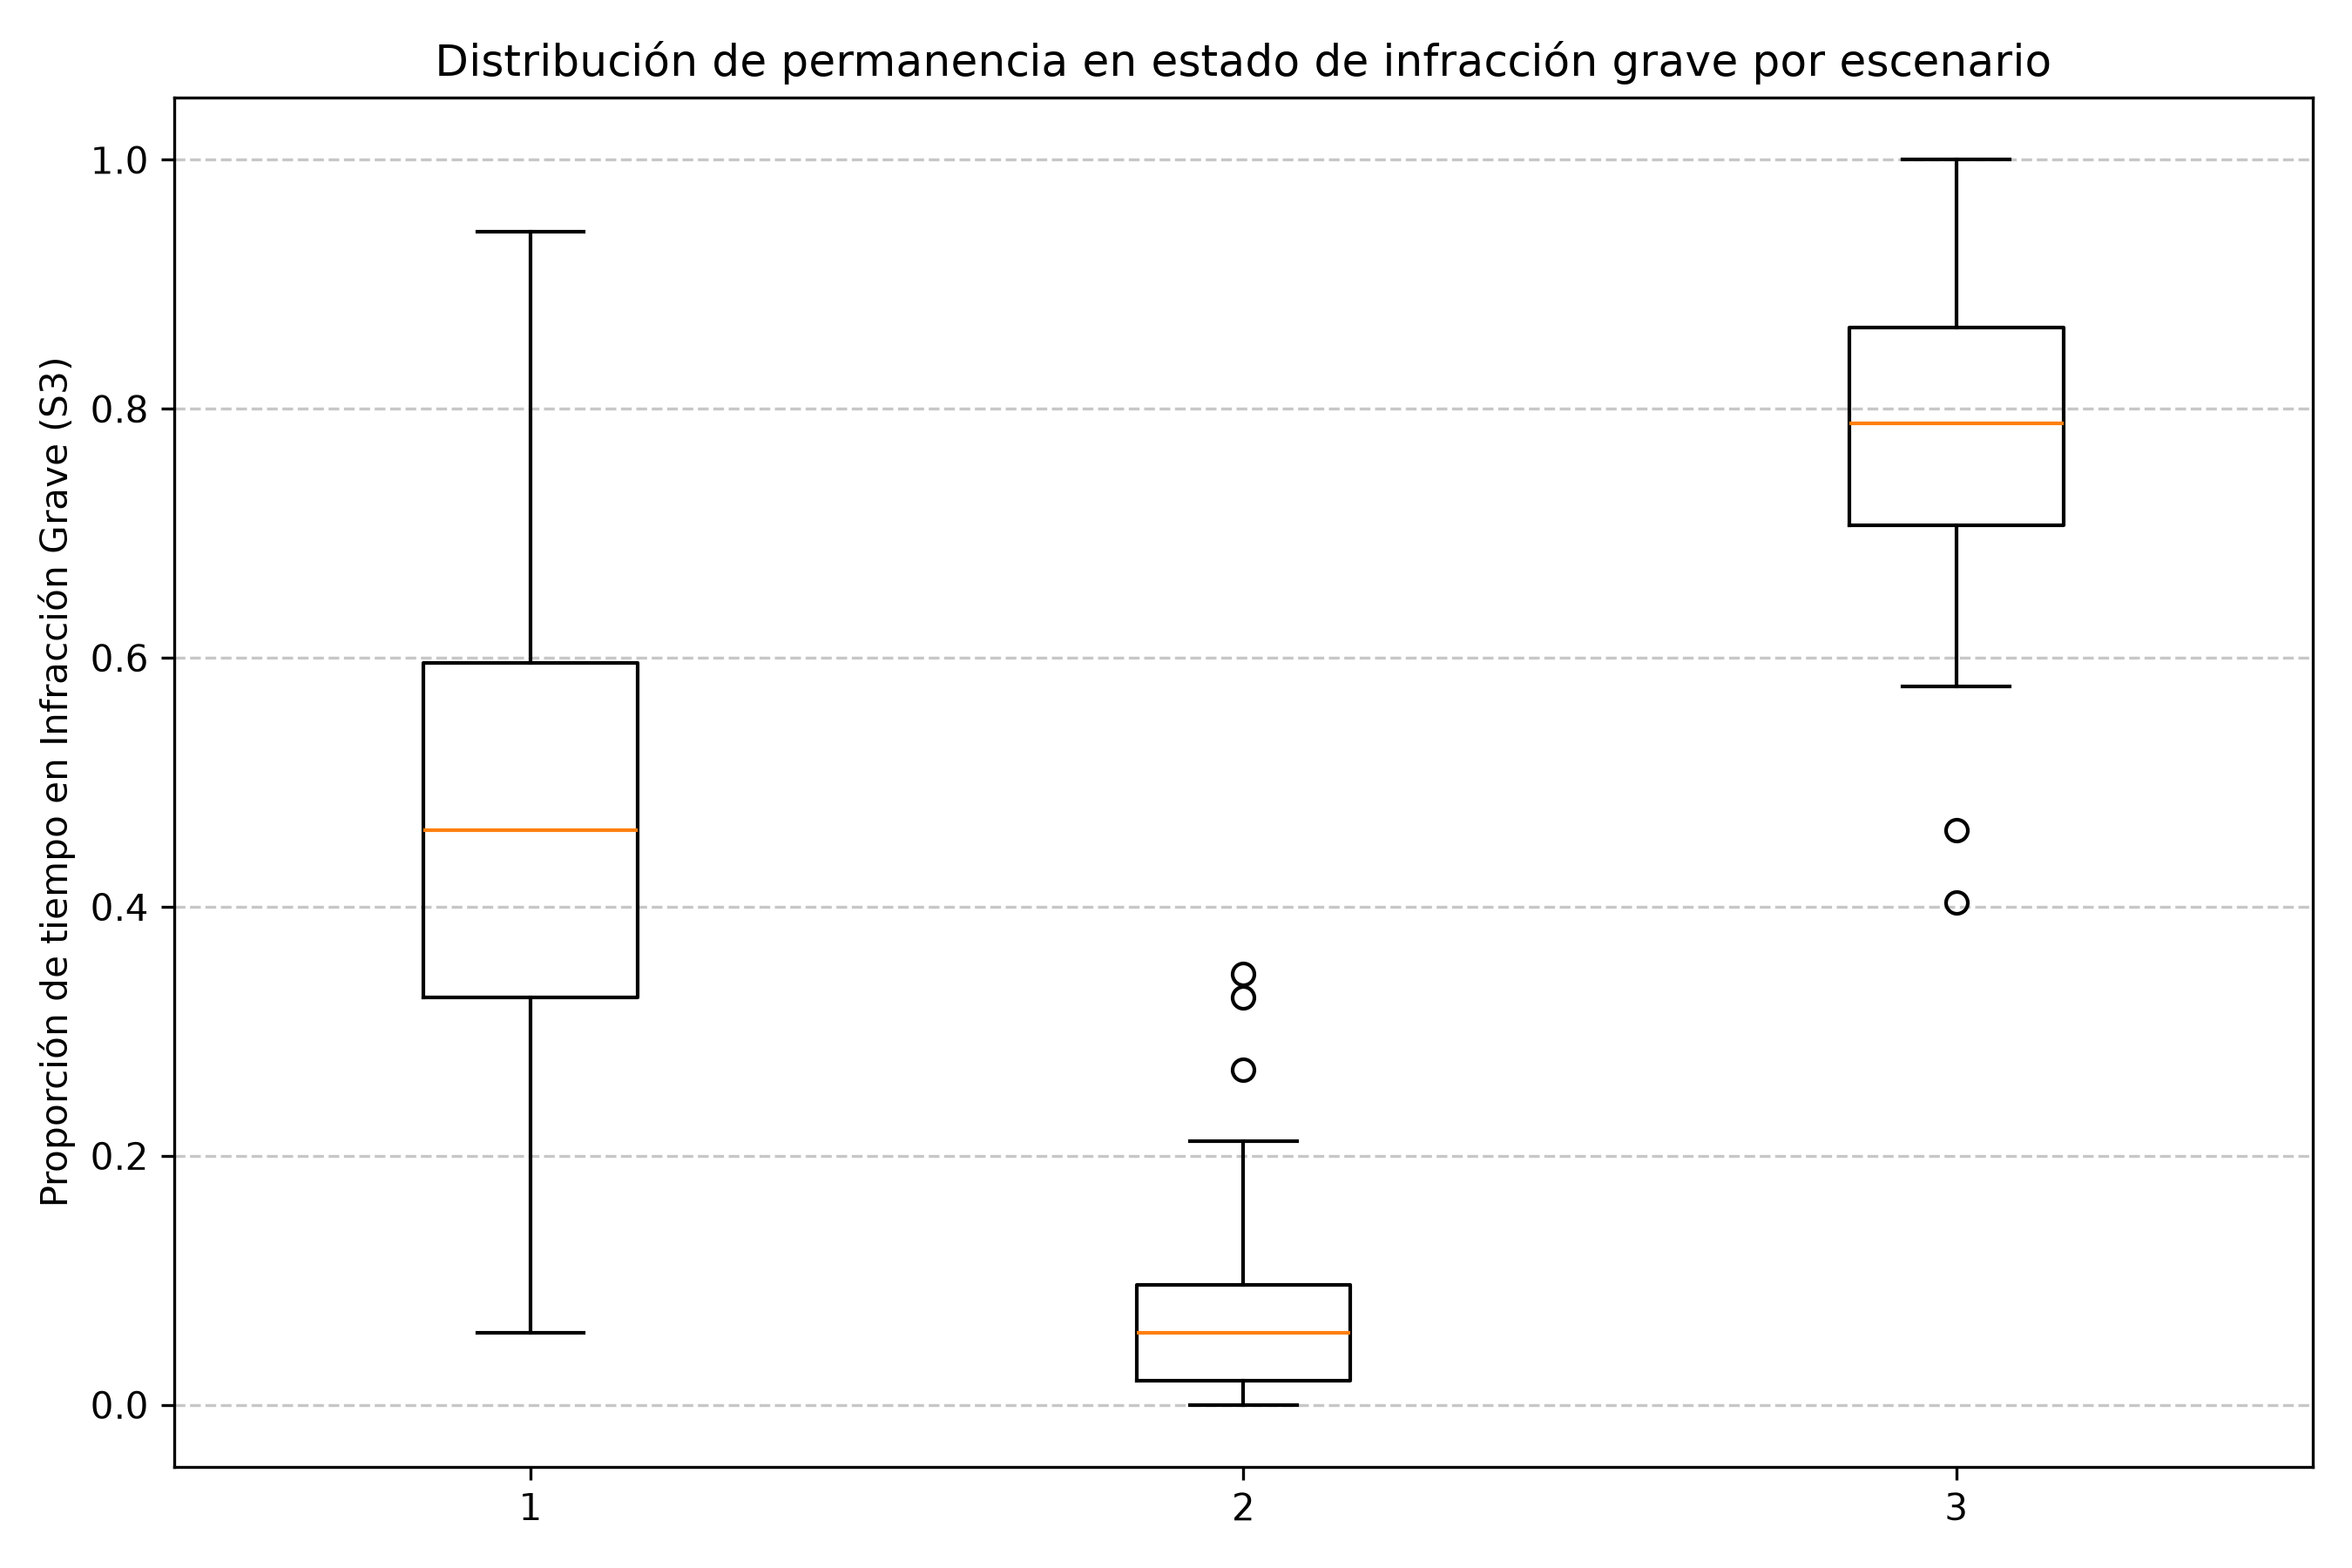
\includegraphics[width=0.85\linewidth]{fig1_boxplot.png}
\caption{Comparación de la distribución de permanencia en infracción grave bajo los tres escenarios de política pública. Generado desde Python con \texttt{matplotlib}.}
\label{fig:boxplot}
\end{figure}

Por otro lado, la evolución probabilística del sistema se representa en la Figura \ref{fig:evolution}. Este gráfico de series de tiempo para el Escenario Base ilustra la dinámica de convergencia propia de las cadenas de Markov. 

Iniciando en un escenario idealista (semana 0), donde el $80\%$ de las obras parten legales ($S_1$), el paso del tiempo y las transiciones naturales del municipio provocan un deterioro. Aproximadamente en la semana 10, la curva de legalidad verde ($S_1$) es intersecada por la curva de infracción roja ($S_3$). Hacia el final del año (semana 50), el sistema se estabiliza mostrando que, con un control base promedio, la ciudad tiende a mantener un 60\% de sus obras en estado de infracción grave de manera estacionaria.

\begin{figure}[H]
\centering
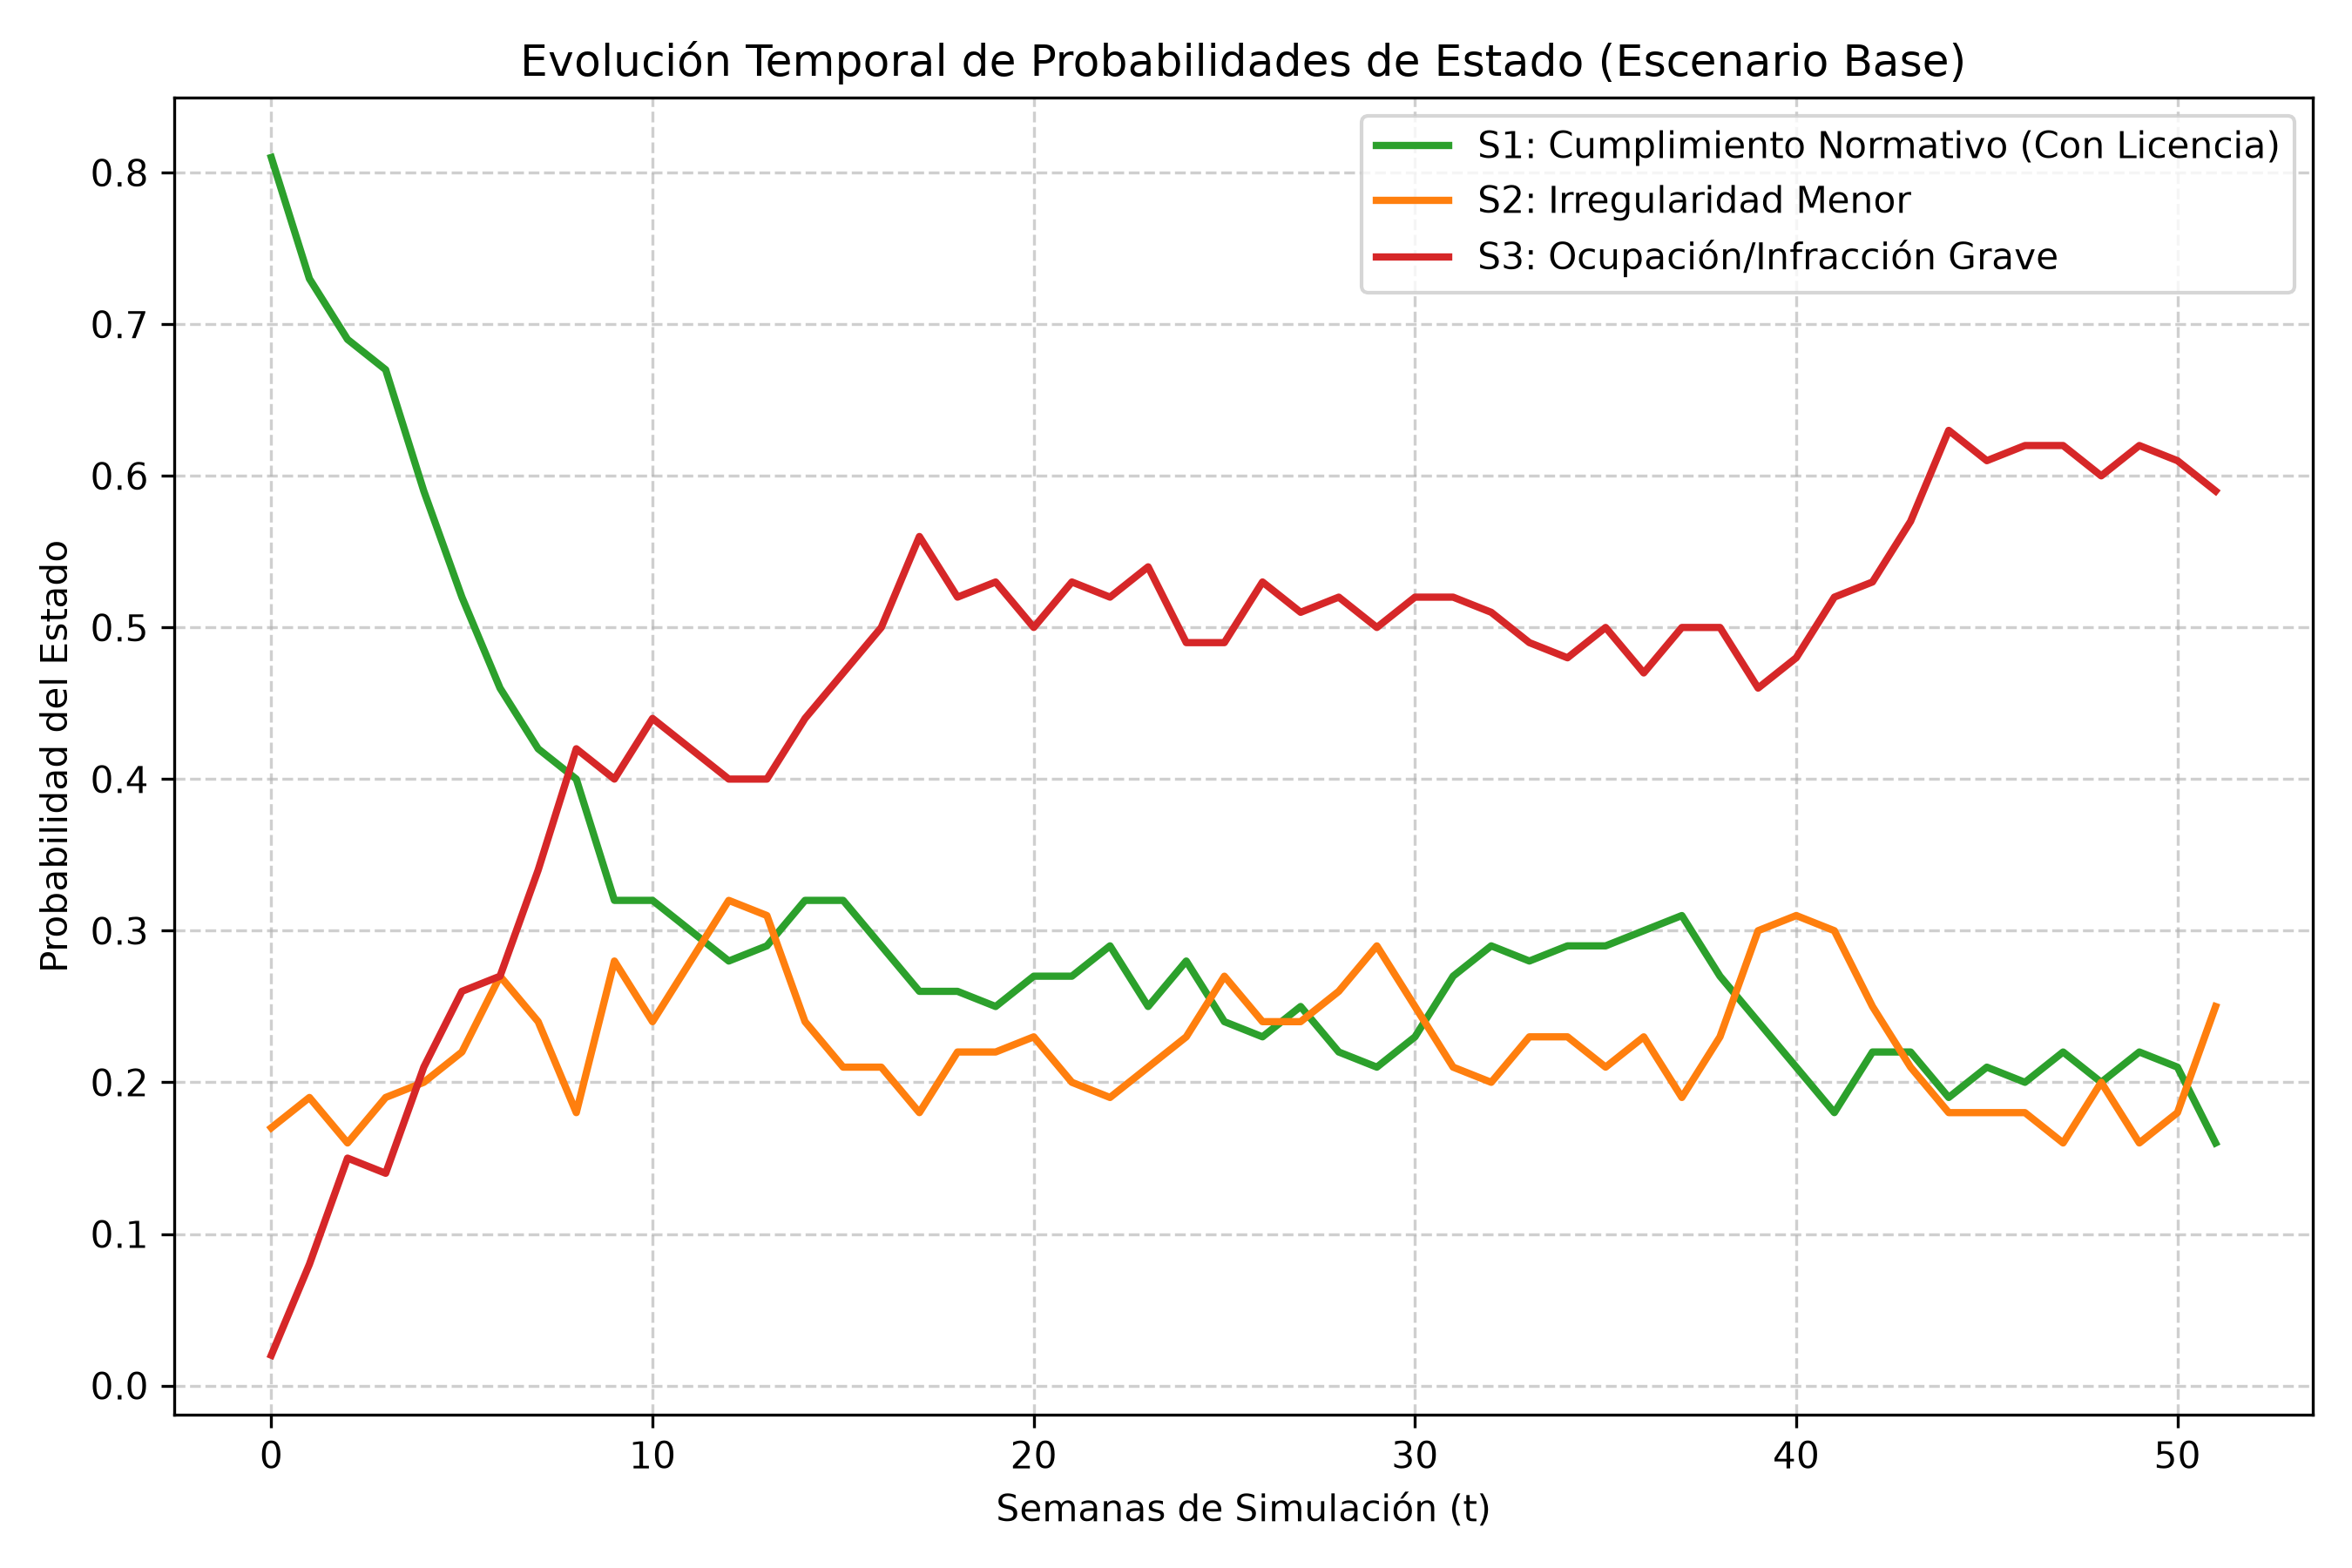
\includegraphics[width=0.85\linewidth]{fig2_evolution.png}
\caption{Evolución temporal de las probabilidades de estado en el escenario base (convergencia estocástica). En verde el cumplimiento normativo; en rojo la consolidación de la infracción grave.}
\label{fig:evolution}
\end{figure}

\section{Discusión}
Los resultados obtenidos corroboran la utilidad pragmática de los Modelos Ocultos de Markov más allá del campo biológico o de telecomunicaciones. El modelo logra capturar la esencia estocástica de la informalidad urbana en Colombia. 

Es imperativo discutir la conexión entre los resultados matemáticos y la gestión pública real. Cuando el modelo opera bajo la matriz de "Control Laxo", el intervalo de confianza [0.755, 0.800] revela un sistema fuera de control: más del 75\% del tiempo la infraestructura se erige violando la Ley 1801 de 2016 y el Decreto 1077 de 2015. Esto representa el escenario típico donde las Secretarías de Infraestructura no cruzan datos oportunamente con las Inspecciones de Policía, permitiendo que la mampostería fragüe y se instalen servicios públicos de forma irregular, lo que posteriormente desencadena engorrosos procesos legales de demolición con acciones de tutela interpuestas por los infractores.

Por el contrario, modificar los parámetros transicionales ($A$) hacia el Escenario Estricto (mediante la inyección de personal técnico y sectorización de visitas de inspección de lunes a viernes) desplomó la permanencia en irregularidades al $7.3\%$ promedio. Esto subraya que la eficiencia administrativa no solo es un mandato legal, sino una variable probabilística capaz de alterar positivamente las series de tiempo del desarrollo municipal.

Comparado con la literatura estudiada [3, 4], nuestra implementación tiene la inmensa ventaja de no requerir software propietario (como ArcGIS o herramientas de visión computacional). Utilizando registros tabulares simples de quejas ciudadanas como secuencias de emisión, el algoritmo es capaz de priorizar cuáles obras deben ser visitadas urgentemente por los técnicos.

\section{Conclusiones y Trabajo Futuro}

Para culminar, se da respuesta sintética y sustentada a las tres preguntas de investigación que guiaron esta simulación:

\begin{itemize}
    \item \textbf{Respuesta a P1:} El desafío de la detección de construcciones ilegales y muros en el espacio público se modeló exitosamente utilizando un HMM. El logro conceptual fue asignar la condición legal de la obra dictada por el Decreto 1077 a los "estados ocultos", y mapear el volumen de quejas ciudadanas y escombros a las "observaciones o emisiones".
    
    \item \textbf{Respuesta a P2:} El impacto de las políticas institucionales es crítico y demostrable probabilísticamente. Ajustar las probabilidades de transición en la simulación (reflejando la inmediatez de respuesta entre la Secretaría de Infraestructura y la Inspección de Convivencia) redujo la media de invasiones del 46.2\% al 7.3\%, confirmando que el control oportuno altera la distribución estacionaria del municipio a largo plazo.
    
    \item \textbf{Respuesta a P3:} El desarrollo algorítmico presentado en este trabajo probó ser totalmente reproducible y estable al configurar parámetros constantes de semilla (\texttt{np.random.seed}). Además, el diagrama de cajas demostró que el modelo es altamente sensible al cambio paramétrico de las matrices, reflejando fielmente la teoría matemática de los procesos estocásticos de primer orden.
\end{itemize}

\textbf{Trabajo Futuro:}
La continuación natural de este estudio será la transición de una "Simulación Paramétrica" a una "Inferencia de Datos Reales". Se propone compilar el registro histórico de los últimos cinco años de los archivos físicos de la Inspección de Policía de un municipio de categoría intermedia (ej. reportes de comparendos bajo la Ley 1801), y utilizar el algoritmo de Baum-Welch para que el modelo entrene y aprenda de forma autónoma las verdaderas matrices de transición $A$ y de emisión $B$ empíricas del territorio.

\begin{thebibliography}{10}

\bibitem{1} L. Rabiner, ``A tutorial on hidden Markov models and selected applications in speech recognition,'' \textit{Proc. IEEE}, vol. 77, no. 2, pp. 257-286, 1989.

\bibitem{2} Ministerio de Vivienda, Ciudad y Territorio. \textit{Decreto 1077 de 2015. Por medio del cual se expide el Decreto Único Reglamentario del Sector Vivienda, Ciudad y Territorio.} Bogotá, Colombia, 2015.

\bibitem{3} Congreso de la República de Colombia. \textit{Ley 1801 de 2016. Por la cual se expide el Código Nacional de Seguridad y Convivencia Ciudadana.} Bogotá, Colombia, 2016.

\bibitem{4} P. Wang, ``Citizen Complaints as Emission Sequences in HMM,'' \textit{J. Urban Planning and Develop.}, vol. 148, no. 3, 2022.

\bibitem{5} C. Ruiz, ``Monitoring Infrastructure Degradation with Hidden States,'' \textit{IEEE Access}, vol. 9, pp. 45012-45023, 2021.

\bibitem{6} K. Lee and S. Park, ``Stochastic Modeling for Smart City Public Space Management,'' \textit{Smart Cities}, vol. 6, no. 1, pp. 200-215, 2023.

\bibitem{7} M. Gómez et al., ``Predicting Unplanned Urban Expansion Using Stochastic Processes,'' \textit{Comput., Environ. and Urban Syst.}, vol. 91, 2022.

\bibitem{8} A. Silva, ``Machine Learning in Municipal Administration,'' \textit{Public Admin. Rev.}, 2023.

\bibitem{9} J. Chen, ``Satellite Image Processing for Illegal Construction Detection,'' \textit{Remote Sens.}, vol. 15, no. 8, 2023.

\bibitem{10} D. Vargas and R. Blanco, ``Data Mining of Municipal Inspection Reports for Predictive Policing,'' \textit{IEEE Int. Conf. on Big Data}, 2022.

\end{thebibliography}

\end{document}